\documentclass[11pt]{article}
\usepackage[margin=0.8in]{geometry}
\usepackage{amsmath,amssymb,mathtools}
\usepackage{booktabs,array,longtable}
\usepackage{enumitem}
\usepackage{xcolor}
\usepackage{graphicx}
\usepackage{float}
\usepackage{adjustbox}
\usepackage{tikz}
\usetikzlibrary{arrows.meta,positioning,shapes.geometric,calc,shapes.arrows}
% Color definitions to match the whiteboard markers (wheel diagram)
\definecolor{wbgreen}{RGB}{0,150,120}
\definecolor{wbblue}{RGB}{40,70,160}
\definecolor{wbred}{RGB}{150,30,30}
\usepackage{hyperref}
\hypersetup{colorlinks=true,linkcolor=blue,urlcolor=blue}
\setlength{\parindent}{0pt}
\setlength{\parskip}{0.55em}
\renewcommand{\arraystretch}{1.18}

\newcommand{\pos}[1]{\left(#1\right)^+}
\newcommand{\Call}{\mathrm{CALL}}
\newcommand{\Put}{\mathrm{PUT}}
\newcommand{\CCR}{\mathrm{CCR}_{S_0}}
\newcommand{\CSPR}{\mathrm{CSPR}_{S_0}}
\newcommand{\BCSR}{\mathrm{BCSR}}
\newcommand{\BPSR}{\mathrm{BPSR}}
% Tranche labels --- full-size identifier with literal underscore (CALL_N, CALL_P, ...)
\newcommand{\CN}{\mathrm{CALL\_N}}
\newcommand{\CP}{\mathrm{CALL\_P}}
\newcommand{\PN}{\mathrm{PUT\_N}}
\newcommand{\PP}{\mathrm{PUT\_P}}
\newcommand{\CNP}{\mathrm{CALL\_NP}}
\newcommand{\CNN}{\mathrm{CALL\_NN}}
\newcommand{\PNP}{\mathrm{PUT\_NP}}
\newcommand{\PNN}{\mathrm{PUT\_NN}}
% Strike-tagged tranche labels: full-size name, strike as a real (smaller) subscript
\newcommand{\CNat}[1]{\mathrm{CALL\_N}_{#1}}
\newcommand{\CPat}[1]{\mathrm{CALL\_P}_{#1}}
\newcommand{\PNat}[1]{\mathrm{PUT\_N}_{#1}}
\newcommand{\PPat}[1]{\mathrm{PUT\_P}_{#1}}
\newcommand{\CNPi}[1]{\mathrm{CALL\_NP}_{#1}}
\newcommand{\CNNi}[1]{\mathrm{CALL\_NN}_{#1}}
\newcommand{\PNPi}[1]{\mathrm{PUT\_NP}_{#1}}
\newcommand{\PNNi}[1]{\mathrm{PUT\_NN}_{#1}}
% Placeholder marker for content still to be drafted (charts / diagrams / tables)
\newcommand{\todo}[1]{\par\medskip\noindent{\color{wbred}\itshape[\textbf{TODO:} #1]}\par\medskip}

\title{Tokenized Option Ladder: Mathematical Formulation}
\author{}
\date{}

\begin{document}
\maketitle
\vspace{-2em}

% =====================================================================
% This document is Section 4 (Math) of the StrikeX white paper.
% Layout:
%   Sec.1  Setup and the Splitting Primitive        (white paper 4.0)
%   Sec.2  Route Strategy Map                        (white paper 4.1)
%   Sec.3  Call Side  (long call / covered call / bull call spread / conservation)
%   Sec.4  Put Side   (long put / cash-secured put / bear put spread / conservation)
%   Sec.5  Wheeling (Reinvest Strategy)              (white paper 4.4)
%   Sec.6  Summary                                   (white paper 4.5)
% Per-strategy template (6 parts):
%   (1) how it works  (2) splitting equation  (3) clearing/settlement equation
%   (4) split+clearing diagram  (5) settlement-vs-price chart  (6) settlement table
% =====================================================================

% =====================================================================
\section{Setup and the Splitting Primitive}
% =====================================================================

\subsection{Mechanism and Prerequisites}

\textbf{Maturity and clearing.} A position is opened against collateral and settled
at a single maturity $m$. At maturity an oracle posts the terminal underlying price
$X_m$ \emph{once}; every tranche then clears to a closed-form cash (or collateral)
amount. The oracle is therefore needed only at this clearing instant, not during the
life of the position.

\textbf{Two collateral states.} Every construction starts from one of two collateral
states: one unit of the underlying $T$ (terminal value $X_m$), or cash $C$ (in the
put-side base split $C=S_0$).

\textbf{Numeraire.} Payoffs are written in cash / numeraire value by default;
collateral-unit forms (underlying-$T$ units, cash units) are given where useful.

\textbf{Scope.} This section is a payoff \emph{decomposition}, not a pricing model.
Premiums are set by the market; the math here only guarantees that the tranches
partition the collateral's terminal value exactly.

\subsection{The Splitting Primitive}

At a chosen strike $S$, any collateral position splits into an \emph{obligation
residual} $P$ and a \emph{right} $N$,
\[
\text{Collateral} \;=\; \underbrace{P}_{\text{residual}} \;+\; \underbrace{N}_{\text{right}},
\qquad
P(X_m)+N(X_m)=\text{(terminal value of the collateral)}\ \ \forall X_m .
\]
This conservation identity is what makes every tranche \emph{fully collateralized}:
the pieces always sum back to the collateral that backs them.

\subsection{Tranche-Address Notation (the \texorpdfstring{$P/N$}{P/N} Tree)}

The suffix on each label is the path taken through the recursion. Starting from the
collateral, every split sends the obligation residual to a leaf ($P$, a tranche the
holder keeps) and keeps splitting the right ($N$):

\begin{center}
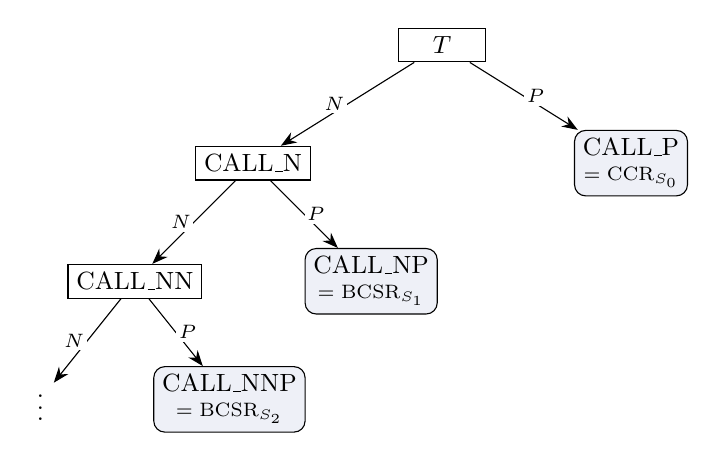
\begin{tikzpicture}[
  font=\small,
  level 1/.style={level distance=15mm, sibling distance=48mm},
  level 2/.style={level distance=15mm, sibling distance=30mm},
  level 3/.style={level distance=15mm, sibling distance=24mm},
  spine/.style={draw, inner sep=3pt, minimum width=11mm},
  leaf/.style={draw, rounded corners, fill=wbblue!8, inner sep=3pt, align=center},
  elab/.style={midway, font=\scriptsize, fill=white, inner sep=1pt},
  edge from parent/.style={draw, -{Stealth[length=2mm]}},
]
\node[spine] {$T$}
  child {node[spine] {$\CN$}
    child {node[spine] {$\CNN$}
      child {node {$\vdots$} edge from parent node[elab,left] {$N$}}
      child {node[leaf] {$\mathrm{CALL\_NNP}$\\[-2pt]{\scriptsize$=\BCSR_{S_2}$}} edge from parent node[elab,right] {$P$}}
      edge from parent node[elab,left] {$N$}
    }
    child {node[leaf] {$\CNP$\\[-2pt]{\scriptsize$=\BCSR_{S_1}$}} edge from parent node[elab,right] {$P$}}
    edge from parent node[elab,left] {$N$}
  }
  child {node[leaf] {$\CP$\\[-2pt]{\scriptsize$=\CCR$}} edge from parent node[elab,right] {$P$}};
\end{tikzpicture}
\end{center}

The strike ladder \emph{is} this recursion. Reading down the right edges gives the menu
of tranches the protocol mints---$\CP$ (the covered-call residual $\CCR$), then
$\CNP,\,\mathrm{CALL\_NNP},\dots$ (the bull-spread residuals $\BCSR_{S_1},\BCSR_{S_2},\dots$)---while
the left spine carries the remaining call right down to the tail call $\Call_{S_n}$. The
running index $i$ flattens the repeated-$N$ path, so $\BCSR_{S_i}$ is the residual produced
at the $i$-th split.

\subsection{Notation}

\begin{longtable}{>{\raggedright\arraybackslash}p{0.23\linewidth}p{0.68\linewidth}}
\toprule
Symbol & Meaning \\
\midrule
$X$ & Spot price of the underlying (running). \\
$X_m$ & Terminal underlying price at maturity $m$, in cash/numeraire units; the one value the oracle posts at clearing. \\
$T$ & One unit of underlying collateral; terminal cash value $X_m$. \\
$C$ & Cash collateral; in the put-side base split $C=S_0$. \\
$S$ & A strike price (generic). \\
$S_i$ & Strike of the $i$-th split, $i=0,\dots,n$; $S_0$ is the base strike. Call ladder: $S_0<S_1<\cdots<S_n$; put ladder: $S_0>S_1>\cdots>S_n$. \\
$N$ & Right leg of a split: the long option right that is split off ($+\Call$ or $+\Put$); the only leg that splits again, i.e.\ the recursing branch of the tree. \\
$P$ & Obligation-residual leg of a split: the collateral the writer keeps after the right $N$ is split off; it carries the short-option obligation. Every split obeys $\text{collateral}=P+N$. \\
$\Call_{S_i}$ & Tokenized call position struck at $S_i$ (a token, not a traded option); terminal value $\max(0,X_m-S_i)$. \\
$\Put_{S_i}$ & Tokenized put position struck at $S_i$ (a token, not a traded option); terminal value $\max(0,S_i-X_m)$. \\
$\pm\Call_{S_i},\ \pm\Put_{S_i}$ & Long ($+$) / short ($-$) the corresponding token. \\
$\mathrm{CC}$ & Covered call (strategy): hold the underlying and write a call against it, capping the upside above the strike in return for the premium. \\
$\CCR$ (CALL\_P) & Covered-call residual token: the base-split residual leg $T-\Call_{S_0}$. Exists only at the base strike $S_0$. \\
$\mathrm{CSP}$ & Cash-secured put (strategy): hold cash and write a put fully backed by that cash, taking on the obligation to buy the underlying below the strike. \\
$\CSPR$ (PUT\_P) & Cash-secured-put residual token: the base-split residual leg $C-\Put_{S_0}$. Exists only at $S_0$. \\
$\mathrm{BCS}$ & Bull call spread (strategy): long $\Call_{S_{i-1}}$, short $\Call_{S_i}$ (the $i$-th rung), a bounded bullish payoff between the two strikes. \\
$\BCSR_{S_i}$ (CALL\_NP) & Bull-call-spread residual token at the $i$-th split ($i=1,\dots,n$): the residual leg of the bull call spread $\mathrm{BCS}$, between strikes $S_{i-1}$ and $S_i$. \\
$\mathrm{BPS}$ & Bear put spread (strategy): long $\Put_{S_{i-1}}$, short $\Put_{S_i}$ (the $i$-th rung), a bounded bearish payoff between the two strikes. \\
$\BPSR_{S_i}$ (PUT\_NP) & Bear-put-spread residual token at the $i$-th split ($i=1,\dots,n$): the residual leg of the bear put spread $\mathrm{BPS}$, between strikes $S_{i-1}$ and $S_i$. \\
\bottomrule
\end{longtable}

\clearpage
% =====================================================================
\section{Route Strategy Map}
% =====================================================================

\begin{figure}[H]
\centering
\adjustbox{max width=\textwidth,max totalheight=0.8\textheight,center}{%
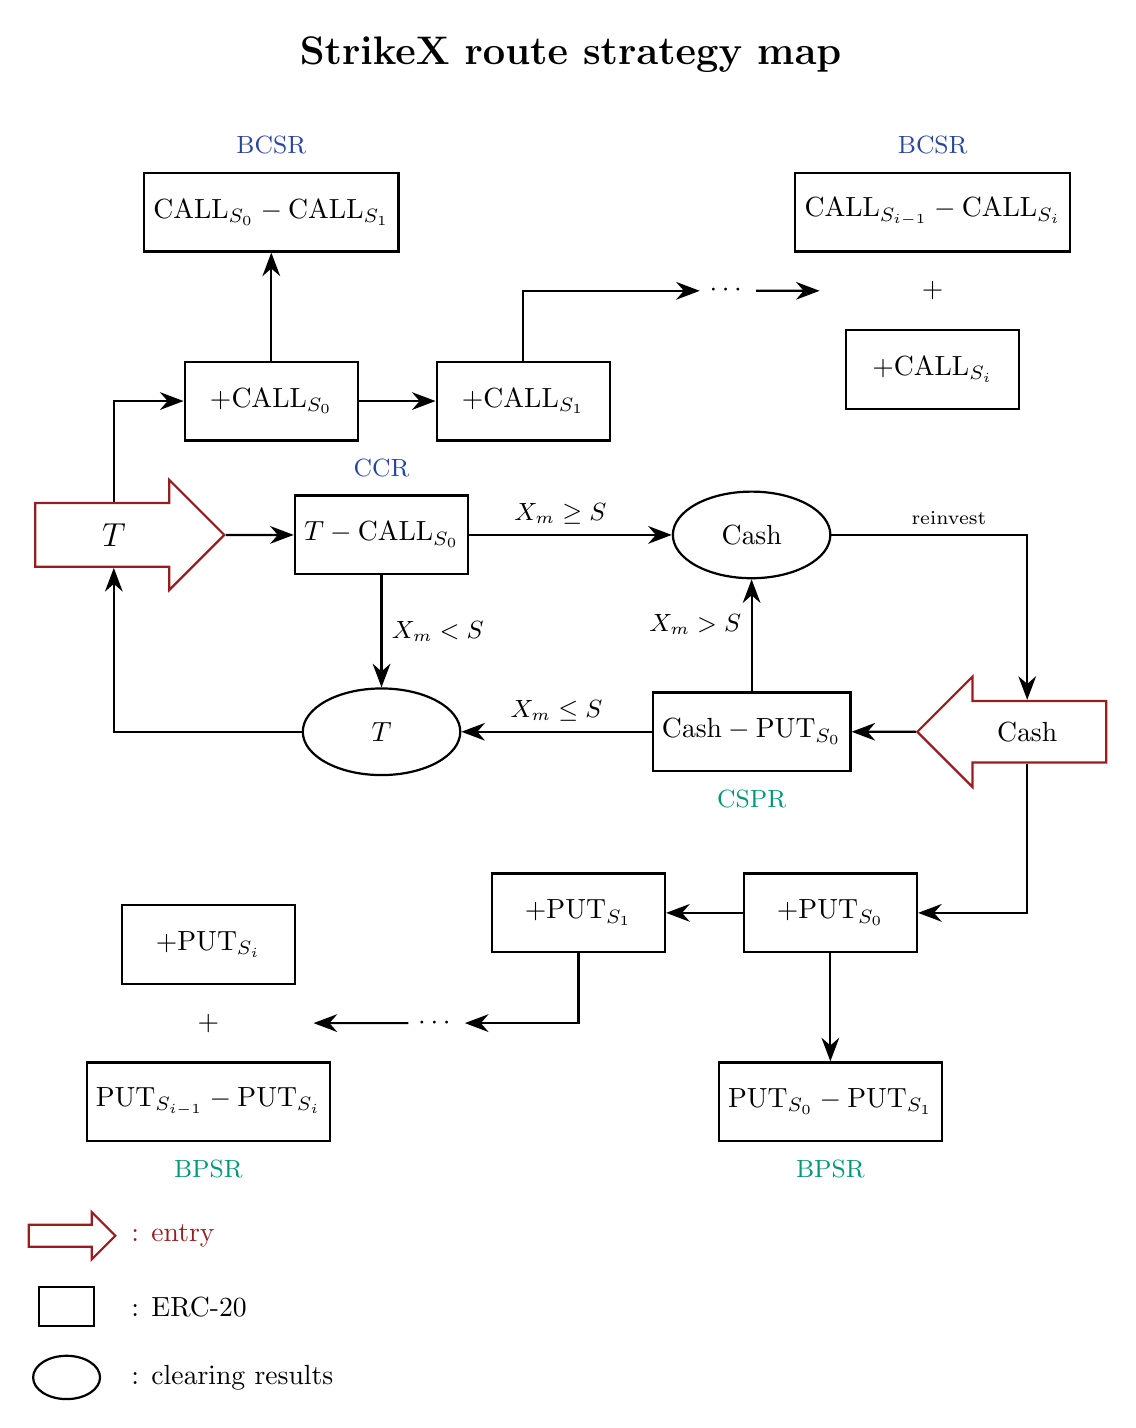
\begin{tikzpicture}[
  font=\sffamily,
  box/.style={draw, rectangle, minimum width=2.2cm, minimum height=1cm, align=center, line width=0.8pt},
  ell/.style={draw, ellipse, minimum width=2cm, minimum height=1.1cm, align=center, line width=0.8pt},
  >={Stealth[length=3mm]},
  arrline/.style={->, line width=0.8pt},
]

% ============ Graph title ============
\node[font=\Large\bfseries] at (6.4,11.0) {StrikeX route strategy map};

% (T base-split equation: moved below the figure)

% ============ BCSR boxes (top) ============
\node[box] (bcsr1) at (2.6,9.0) {$\mathrm{CALL}_{S_0}-\mathrm{CALL}_{S_1}$};
\node[align=center, font=\small, color=wbblue] at (2.6,9.85) {BCSR};

\node[box] (bcsr2top) at (11.0,9.0) {$\mathrm{CALL}_{S_{i-1}}-\mathrm{CALL}_{S_i}$};
\node[align=center, font=\small, color=wbblue] at (11.0,9.85) {BCSR};
\node[box] (bcsr2bot) at (11.0,7.0) {$+\mathrm{CALL}_{S_i}$};
\node at (11.0,8.0) {$+$};

% (CALL-NP / CALL-NN payoffs: moved below the figure)

% ============ +CALL boxes (middle-upper) ============
\node[box] (callS0) at (2.6,6.6) {$+\mathrm{CALL}_{S_0}$};
\node[box] (callS1) at (5.8,6.6) {$+\mathrm{CALL}_{S_1}$};

% ============ Entry arrow T (big arrow, left) ============
\node[single arrow, draw, line width=0.8pt, minimum width=1.4cm, minimum height=2.4cm,
      single arrow head extend=2mm, color=wbred, rotate=0] (Tentry) at (0.6,4.9) {\color{black}\large $T$};

% ============ CCR: T - CALL_S0 ============
\node[box] (ccr) at (4.0,4.9) {$T-\mathrm{CALL}_{S_0}$};
\node[align=center, font=\small, color=wbblue] at (4.0,5.75) {CCR};

% ============ Cash ellipse ============
\node[ell] (cash1) at (8.7,4.9) {$\mathrm{Cash}$};

% ============ T ellipse (lower) ============
\node[ell] (Tell) at (4.0,2.4) {$T$};

% ============ CSPR: Cash - PUT_S0 ============
\node[box] (cspr) at (8.7,2.4) {$\mathrm{Cash}-\mathrm{PUT}_{S_0}$};
\node[align=center, font=\small, color=wbgreen] at (8.7,1.55) {CSPR};

% ============ Cash entry arrow (right) ============
\node[single arrow, draw, line width=0.8pt, minimum width=1.4cm, minimum height=2.4cm,
      single arrow head extend=2mm, color=wbred, shape border rotate=180] (cashentry) at (12.2,2.4) {\color{black}$\mathrm{Cash}$};

% ============ +PUT boxes ============
\node[box] (putS0) at (9.7,0.1) {$+\mathrm{PUT}_{S_0}$};
\node[box] (putS1) at (6.5,0.1) {$+\mathrm{PUT}_{S_1}$};
\node[box] (bpsr1) at (9.7,-2.3) {$\mathrm{PUT}_{S_0}-\mathrm{PUT}_{S_1}$};
\node[align=center, font=\small, color=wbgreen] at (9.7,-3.15) {BPSR};

% ============ General-step vertical stack (+PUT_Si over PUT_{Si-1}-PUT_Si) ============
\node[box] (putSi) at (1.8,-0.3) {$+\mathrm{PUT}_{S_i}$};
\node at (1.8,-1.3) {$+$};
\node[box] (bpsr2) at (1.8,-2.3) {$\mathrm{PUT}_{S_{i-1}}-\mathrm{PUT}_{S_i}$};
\node[align=center, font=\small, color=wbgreen] at (1.8,-3.15) {BPSR};

% (Cash base-split equation: moved below the figure)

% (PUT-NP / PUT-NN payoffs: moved below the figure)

% ===================== ARROWS =====================

% +CALL_{S_0} fans out: spread residual (CALL_{S_0}-CALL_{S_1}) and carry (+CALL_{S_1})
\draw[arrline] (callS0) -- (callS1);
\draw[arrline] (callS0.north) -- (bcsr1.south);
% +CALL_{S_1} -> up then right (90 deg) -> ... -> middle of the general-step stack
\node (ccdots) at (8.4,8.0) {$\cdots$};
\draw[arrline] (callS1.north) |- (ccdots.west);
\draw[arrline] (ccdots.east) -- ($(bcsr2top.west)!0.5!(bcsr2bot.west)$);

% Entry T arrow up to +CALL_S0   (label C.N)
\draw[arrline] (Tentry.north) |- node[pos=0.25, left, font=\small] {} (callS0.west);
% (C.N entry weight: moved below the figure)

% Entry T -> CCR box (label C.P) -- the lower split going right into T-CALL
\draw[arrline] (Tentry.east) -- (ccr.west);

% CCR -> Cash  (Xm >= S)
\draw[arrline] (ccr.east) -- node[pos=0.45, above, font=\small] {$X_m\ge S$} (cash1.west);

% CCR -> T ellipse (Xm < S)  downward
\draw[arrline] (ccr.south) -- node[pos=0.5, right, font=\small] {$X_m<S$} (Tell.north);

% Cash clearing result reinvested via the cash entry
\draw[arrline] (cash1.east) -| node[pos=0.3,above,font=\scriptsize]{reinvest} (cashentry.north);

% cashentry -> CSPR  (P.P label)
\draw[arrline] (cashentry.west) -- (cspr.east);

% CSPR -> T ellipse  (Xm <= S)
\draw[arrline] (cspr.west) -- node[pos=0.5, above, font=\small] {$X_m\le S$} (Tell.east);

% CSPR -> Cash (Xm > S) upward green
\draw[arrline] (cspr.north) -- node[pos=0.6, left, font=\small] {$X_m>S$} (cash1.south);

% cashentry -> +PUT_S0 (P.N label)
\draw[arrline] (cashentry.south) |- node[pos=0.25, right, font=\small] {} (putS0.east);
% (P.N entry weight: moved below the figure)

% putS0 -> left -> putS1
\draw[arrline] (putS0.west) -- (putS1.east);
% putS0 -> straight down -> middle of bpsr1
\draw[arrline] (putS0.south) -- (bpsr1.north);
% +PUT_{S_1} -> down then left (90 deg) -> ... -> middle of the general-step stack
\node (pcdots) at (4.7,-1.3) {$\cdots$};
\draw[arrline] (putS1.south) |- (pcdots.east);
\draw[arrline] (pcdots.west) -- ($(putSi.east)!0.5!(bpsr2.east)$);

% Tell -> back to entry T (blue feedback loop, lower)
\draw[arrline] (Tell.west) -| (Tentry.south);

% (removed return path: keep a single arrow T -> +CALL_{S_0})

% ===================== LEGEND (bottom-left) =====================
\begin{scope}[shift={(0,-4.0)},font=\rmfamily]
  \node[single arrow, draw, color=wbred, line width=0.8pt, minimum width=0.6cm,
        minimum height=1.1cm, single arrow head extend=1.5mm] (le) at (0,0) {};
  \node[anchor=west, color=wbred] at (0.7,0) {: entry};
  \node[draw, rectangle, line width=0.8pt, minimum width=0.7cm, minimum height=0.5cm] at (0,-0.9) {};
  \node[anchor=west] at (0.7,-0.9) {: ERC-20};
  \node[draw, ellipse, line width=0.8pt, minimum width=0.85cm, minimum height=0.55cm] at (0,-1.8) {};
  \node[anchor=west] at (0.7,-1.8) {: clearing results};
\end{scope}

\end{tikzpicture}%
}
\caption{Route strategy map. From each collateral state, the base split yields an
obligation residual ($P$, the $\CCR$/$\CSPR$ token) and a right ($N$); the residuals
settle to cash or $T$ at maturity according to $X_m$ vs.\ the strike $S$, while the
rights recurse along the strike ladder into the vertical-spread residuals
$\BCSR$/$\BPSR$.}
\label{fig:routemap}
\end{figure}

Figure~\ref{fig:routemap} indexes the whole construction: each strategy of Sections~3--4
is one labeled route on this map, and Section~5 reads the same graph as a reinvestment
cycle.

% =====================================================================
\section{Long Underlying Assets}
% =====================================================================

A long position in the underlying $T$ (terminal value $X_m$) is tokenized into a ladder
of call-side tranches. The base split (Section~3.1) carves $T$ into a long-call token and
a covered-call residual; the recursive split (Section~3.2) carves the long-call token into
bull-call-spread tranches along the strike ladder; and the whole ladder conserves back to
$X_m$ (Section~3.3).

% ---------------------------------------------------------------------
\subsection{Call-Side Base Split \& Covered Call}
% ---------------------------------------------------------------------

\begin{center}
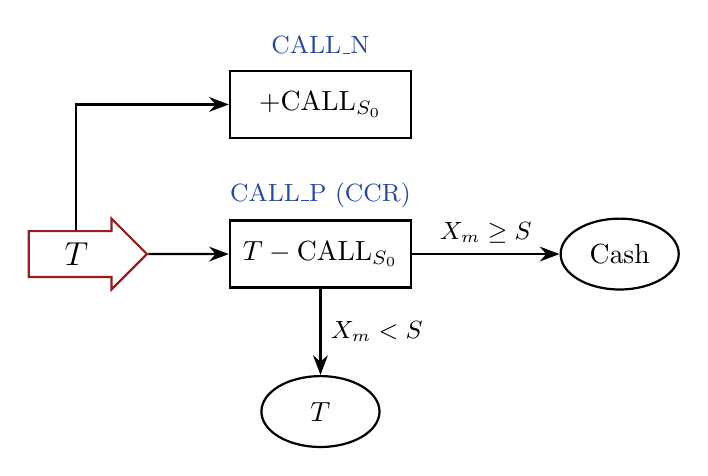
\begin{tikzpicture}[
  font=\sffamily,
  box/.style={draw, rectangle, minimum width=2.3cm, minimum height=0.85cm, align=center, line width=0.8pt},
  ell/.style={draw, ellipse, minimum width=1.5cm, minimum height=0.9cm, align=center, line width=0.8pt},
  >={Stealth[length=2.5mm]},
  arrline/.style={->, line width=0.8pt},
]
\node[single arrow, draw, line width=0.8pt, minimum width=0.9cm, minimum height=1.5cm,
      single arrow head extend=1.5mm, color=wbred] (Tentry) at (0,1.3) {\color{black}\large $T$};
\node[box] (callS0) at (3.1,3.2) {$+\mathrm{CALL}_{S_0}$};
\node[font=\small, color=wbblue] at (3.1,3.95) {$\CN$};
\node[box] (ccr) at (3.1,1.3) {$T-\mathrm{CALL}_{S_0}$};
\node[font=\small, color=wbblue] at (3.1,2.05) {$\CP$ (CCR)};
\node[ell] (cash1) at (6.9,1.3) {$\mathrm{Cash}$};
\node[ell] (Tell) at (3.1,-0.7) {$T$};
\draw[arrline] (Tentry.north) |- (callS0.west);
\draw[arrline] (Tentry.east) -- (ccr.west);
\draw[arrline] (ccr.east) -- node[pos=0.5,above,font=\small] {$X_m\ge S$} (cash1.west);
\draw[arrline] (ccr.south) -- node[pos=0.5,right,font=\small] {$X_m<S$} (Tell.north);
\end{tikzpicture}
\end{center}

We start \emph{long the underlying}: one unit of collateral $T$, worth $X_m$ at maturity.
At the base strike $S_0$ this long position is tokenized into two ERC-20 tranches---a right
$N$ and a residual $P$:
\[
T = (N,P) \;\longmapsto\; \CN\ \text{(long-call token)} \;+\; \CP\ \text{(covered-call residual)} .
\]

\textbf{(a) Splitting.} At $S_0$ the underlying splits into the covered-call residual (the
underlying minus the written call) and the call right:
\begin{align}
T &= (T-\Call_{S_0}) + \Call_{S_0},\\
T &= \CPat{S_0} + \CNat{S_0}.
\end{align}
$\CPat{S_0}=T-\Call_{S_0}$ is the covered-call leg---long the underlying, short the $S_0$
call, so its upside is capped at $S_0$. $\CNat{S_0}=\Call_{S_0}$ is the long-call leg---the
uncapped upside above $S_0$, collateralized by the residual holder.

\textbf{(b) Settlement.} At maturity each token clears to a closed form:
\begin{align}
\CNat{S_0}(X_m) &= \pos{X_m-S_0}=\max(0,X_m-S_0),\\
\CPat{S_0}(X_m) &= X_m-\pos{X_m-S_0}=\min(X_m,S_0).
\end{align}
The covered-call leg converts the underlying into cash $S_0$ when the call is assigned
($X_m\ge S_0$) and keeps the underlying $T$, worth $X_m$, otherwise. The two legs conserve:
\begin{align}
\CPat{S_0}(X_m)+\CNat{S_0}(X_m)=\min(X_m,S_0)+\pos{X_m-S_0}=X_m.
\end{align}
In underlying-collateral units ($X_m>0$),
\[
\CPat{S_0}^{\,T}=\min\!\left(1,\tfrac{S_0}{X_m}\right)T,
\qquad
\CNat{S_0}^{\,T}=\max\!\left(0,1-\tfrac{S_0}{X_m}\right)T.
\]

\textbf{(c) Settlement charts.} The two legs are the standard long-call and covered-call
payoffs (USD settlement value vs.\ underlying price $X_m$):

\begin{center}
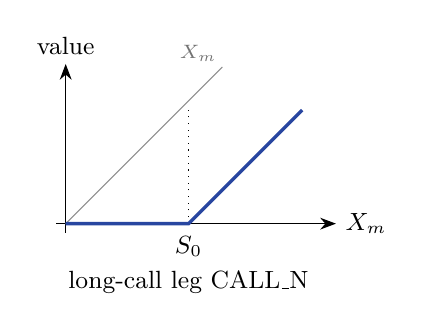
\begin{tikzpicture}[scale=0.78,>={Stealth[length=2mm]},font=\small]
  \draw[->] (-0.15,0) -- (4.4,0) node[right]{$X_m$};
  \draw[->] (0,-0.15) -- (0,2.6) node[above]{value};
  \draw[black!45] (0,0) -- (2.55,2.55) node[black!55,font=\scriptsize,above left=-2pt]{$X_m$};
  \draw[dotted] (2,0) -- (2,1.85);
  \node[below] at (2,-0.05) {$S_0$};
  \draw[wbblue,very thick] (0,0) -- (2,0) -- (3.85,1.85);
  \node[below] at (2.0,-0.62) {long-call leg $\CN$};
\end{tikzpicture}
\hspace{0.9cm}
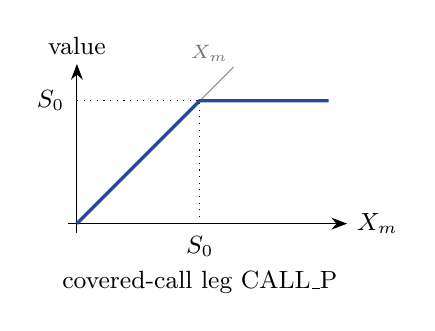
\begin{tikzpicture}[scale=0.78,>={Stealth[length=2mm]},font=\small]
  \draw[->] (-0.15,0) -- (4.4,0) node[right]{$X_m$};
  \draw[->] (0,-0.15) -- (0,2.6) node[above]{value};
  \draw[black!45] (0,0) -- (2.55,2.55) node[black!55,font=\scriptsize,above left=-2pt]{$X_m$};
  \draw[dotted] (2,0) -- (2,2);
  \draw[dotted] (0,2) -- (2,2);
  \node[below] at (2,-0.05) {$S_0$};
  \node[left] at (-0.05,2) {$S_0$};
  \draw[wbblue,very thick] (0,0) -- (2,2) -- (4.1,2);
  \node[below] at (2.0,-0.62) {covered-call leg $\CP$};
\end{tikzpicture}
\end{center}

% ---------------------------------------------------------------------
\subsection{Call-Side Recursive Split \& Bull Call Spread}
% ---------------------------------------------------------------------

\begin{center}
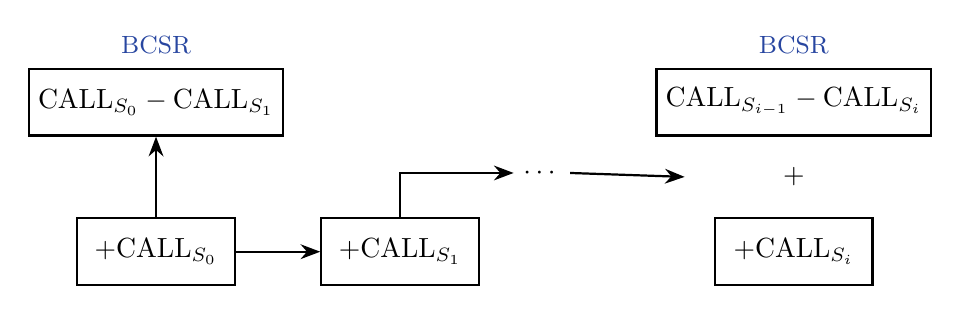
\begin{tikzpicture}[
  font=\sffamily,
  box/.style={draw, rectangle, minimum width=2.0cm, minimum height=0.85cm, align=center, line width=0.8pt},
  >={Stealth[length=2.5mm]},
  arrline/.style={->, line width=0.8pt},
]
\node[box] (callS0) at (0,0) {$+\mathrm{CALL}_{S_0}$};
\node[box] (bcsr1) at (0,1.9) {$\mathrm{CALL}_{S_0}-\mathrm{CALL}_{S_1}$};
\node[font=\small,color=wbblue] at (0,2.62) {BCSR};
\node[box] (callS1) at (3.1,0) {$+\mathrm{CALL}_{S_1}$};
\node (ccdots) at (4.9,1.0) {$\cdots$};
\node[box] (bcsr2top) at (8.1,1.9) {$\mathrm{CALL}_{S_{i-1}}-\mathrm{CALL}_{S_i}$};
\node[font=\small,color=wbblue] at (8.1,2.62) {BCSR};
\node[box] (bcsr2bot) at (8.1,0) {$+\mathrm{CALL}_{S_i}$};
\node at (8.1,0.95) {$+$};
\draw[arrline] (callS0.east) -- (callS1.west);
\draw[arrline] (callS0.north) -- (bcsr1.south);
\draw[arrline] (callS1.north) |- (ccdots.west);
\draw[arrline] (ccdots.east) -- ($(bcsr2top.west)!0.5!(bcsr2bot.west)$);
\end{tikzpicture}
\end{center}

The long-call token $\CN$ is itself split at the next rung. For a call ladder with
increasing strikes $S_0<S_1<\cdots<S_n$, each lower-strike call right splits into a capped
bull-call-spread residual plus the higher-strike call carried further down the ladder. The
call right is tokenized into a further right $N$ and a residual $P$:
\[
\CN = (N,P) \;\longmapsto\; \CNN\ \text{(higher-strike tail call)} \;+\; \CNP\ \text{(bull-call-spread residual)} .
\]

\textbf{(a) Splitting.} For $i=0,\dots,n-1$, the call right $\CNat{S_i}$ is split at the
next strike $S_{i+1}$:
\begin{align}
\CNat{S_i} &=(\Call_{S_i}-\Call_{S_{i+1}})+\Call_{S_{i+1}},\\
\CNat{S_i} &=\CNPi{S_{i+1}}+\CNNi{S_{i+1}}.
\end{align}
$\CNPi{S_{i+1}}$ is the bull-call-spread residual (long the $S_i$ call, short the
$S_{i+1}$ call); $\CNNi{S_{i+1}}$ is the higher-strike tail call --- itself the call
right $\CNat{S_{i+1}}$ handed to the next rung, which splits again.

\textbf{(b) Settlement.}
\begin{align}
\CNPi{S_{i+1}}(X_m) &=\pos{X_m-S_i}-\pos{X_m-S_{i+1}}
=\min\!\left(\max(0,X_m-S_i),\,S_{i+1}-S_i\right),\\
\CNNi{S_{i+1}}(X_m) &=\pos{X_m-S_{i+1}}=\max(0,X_m-S_{i+1}).
\end{align}
Since $S_{i+1}-S_i>0$, the spread residual is non-negative and capped at $S_{i+1}-S_i$.

\textbf{(c) Settlement charts.} The bull-spread leg is capped between adjacent strikes; the
tail call is an ordinary long call struck at $S_{i+1}$:

\begin{center}
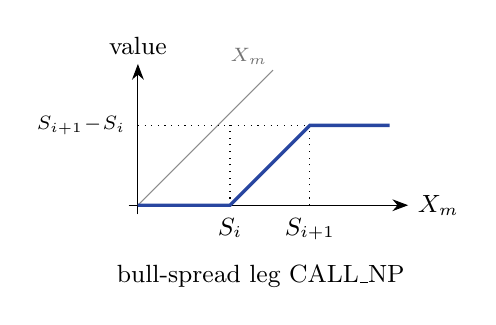
\begin{tikzpicture}[scale=0.78,>={Stealth[length=2mm]},font=\small]
  \draw[->] (-0.15,0) -- (4.4,0) node[right]{$X_m$};
  \draw[->] (0,-0.15) -- (0,2.3) node[above]{value};
  \draw[black!45] (0,0) -- (2.2,2.2) node[black!55,font=\scriptsize,above left=-2pt]{$X_m$};
  \draw[dotted] (1.5,0) -- (1.5,1.3);
  \draw[dotted] (2.8,0) -- (2.8,1.3);
  \draw[dotted] (0,1.3) -- (2.8,1.3);
  \node[below] at (1.5,-0.05) {$S_i$};
  \node[below] at (2.8,-0.05) {$S_{i+1}$};
  \node[left] at (-0.05,1.3) {\scriptsize $S_{i+1}\!-\!S_i$};
  \draw[wbblue,very thick] (0,0) -- (1.5,0) -- (2.8,1.3) -- (4.1,1.3);
  \node[below,align=center] at (2.0,-0.82) {bull-spread leg $\CNP$};
\end{tikzpicture}
\hspace{0.9cm}
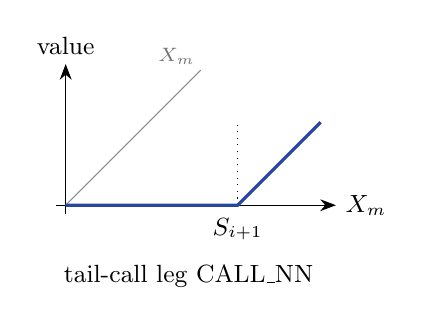
\begin{tikzpicture}[scale=0.78,>={Stealth[length=2mm]},font=\small]
  \draw[->] (-0.15,0) -- (4.4,0) node[right]{$X_m$};
  \draw[->] (0,-0.15) -- (0,2.3) node[above]{value};
  \draw[black!45] (0,0) -- (2.2,2.2) node[black!55,font=\scriptsize,above left=-2pt]{$X_m$};
  \draw[dotted] (2.8,0) -- (2.8,1.3);
  \node[below] at (2.8,-0.05) {$S_{i+1}$};
  \draw[wbblue,very thick] (0,0) -- (2.8,0) -- (4.15,1.35);
  \node[below,align=center] at (2.0,-0.82) {tail-call leg $\CNN$};
\end{tikzpicture}
\end{center}

% ---------------------------------------------------------------------
\subsection{Call-Side Conservation: Combined Chart and Table}
% ---------------------------------------------------------------------

After recursively splitting to $S_n$, the full call-side ladder identity is
\begin{align}
X_m
&=\CCR(X_m)+\sum_{i=1}^{n}\BCSR_{S_i}(X_m)+\Call_{S_n}(X_m),\\
&=\min(X_m,S_0)
+\sum_{i=1}^{n}\left[\pos{X_m-S_{i-1}}-\pos{X_m-S_i}\right]
+\pos{X_m-S_n},\\
&=\min(X_m,S_0)
+\sum_{i=1}^{n}\min\!\left(\max(0,X_m-S_{i-1}),S_i-S_{i-1}\right)
+\max(0,X_m-S_n).
\end{align}
The right-leg sum is telescoping:
\begin{align}
\sum_{i=1}^{n}\left[\pos{X_m-S_{i-1}}-\pos{X_m-S_i}\right]
+\pos{X_m-S_n}
=\pos{X_m-S_0},
\end{align}
so $\min(X_m,S_0)+\pos{X_m-S_0}=X_m$: the tranches always sum back to the underlying.

\textbf{Numerical check.} Parameters $S_0=2000$, $S_1=2500$, with
\begin{align}
\CP &=\min(X_m,2000),\\
\CNP &=\min\!\left(\max(0,X_m-2000),500\right),\\
\CNN &=\max(0,X_m-2500).
\end{align}

\begin{center}
\begin{tabular}{rrrrr}
\toprule
$X_m$ & $\CP$ & $\CNP$ & $\CNN$ & Total \\
\midrule
3600 & 2000 & 500 & 1100 & 3600 \\
2600 & 2000 & 500 & 100 & 2600 \\
2500 & 2000 & 500 & 0 & 2500 \\
2000 & 2000 & 0 & 0 & 2000 \\
1700 & 1700 & 0 & 0 & 1700 \\
1500 & 1500 & 0 & 0 & 1500 \\
1000 & 1000 & 0 & 0 & 1000 \\
\bottomrule
\end{tabular}
\end{center}

\textbf{Combined chart.} Stacking the tokens at every price fills exactly up to the
$45^\circ$ line $X_m$ --- the visual statement of conservation ($S_0=2000$, $S_1=2500$):

\begin{center}
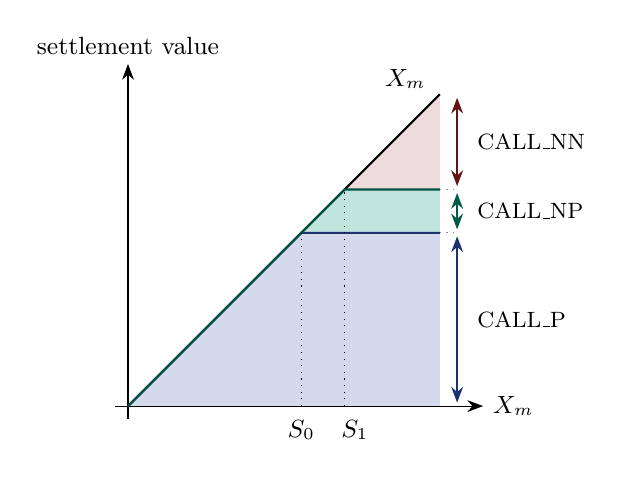
\begin{tikzpicture}[scale=1.1,>={Stealth[length=2mm]},font=\small]
  % stacked bands (cumulative): CALL_P, then +CALL_NP, then +CALL_NN = X_m
  \fill[wbblue!20]  (0,0) -- (2,2) -- (3.6,2) -- (3.6,0) -- cycle;
  \fill[wbgreen!25] (0,0) -- (2,2) -- (3.6,2) -- (3.6,2.5) -- (2.5,2.5) -- cycle;
  \fill[wbred!16]   (0,0) -- (2.5,2.5) -- (3.6,2.5) -- (3.6,3.6) -- cycle;
  % axes
  \draw[->] (-0.15,0) -- (4.1,0) node[right]{$X_m$};
  \draw[->] (0,-0.15) -- (0,3.95) node[above]{settlement value};
  % total (45 degrees)
  \draw[black,thick] (0,0) -- (3.6,3.6);
  \node[above left] at (3.55,3.55) {$X_m$};
  % cumulative boundary lines
  \draw[wbblue!70!black,thick] (0,0) -- (2,2) -- (3.6,2);
  \draw[wbgreen!55!black,thick] (0,0) -- (2.5,2.5) -- (3.6,2.5);
  % strike ticks
  \draw[dotted] (2,0) -- (2,2);   \node[below] at (2,-0.05) {$S_0$};
  \draw[dotted] (2.5,0) -- (2.5,2.5); \node[below] at (2.62,-0.05) {$S_1$};
  % band labels
  % each token's USD claim = its band height, shown as a vertical range bar at the right edge
  \draw[dotted,black!45] (3.6,2)   -- (3.82,2);
  \draw[dotted,black!45] (3.6,2.5) -- (3.82,2.5);
  \draw[<->,wbblue!70!black,line width=0.8pt]  (3.8,0.04) -- (3.8,1.96);
  \node[anchor=west,font=\footnotesize] at (3.92,1.0)  {$\CP$};
  \draw[<->,wbgreen!60!black,line width=0.8pt] (3.8,2.04) -- (3.8,2.46);
  \node[anchor=west,font=\footnotesize] at (3.92,2.25) {$\CNP$};
  \draw[<->,wbred!65!black,line width=0.8pt]   (3.8,2.54) -- (3.8,3.56);
  \node[anchor=west,font=\footnotesize] at (3.92,3.05) {$\CNN$};
\end{tikzpicture}
\end{center}

% =====================================================================
\section{Short Underlying Assets}
% =====================================================================

A cash position $C=S_0$ --- the bearish, ``short'' side --- is tokenized into a ladder of
put-side tranches. The base split (Section~4.1) carves the cash into a long-put token and a
cash-secured-put residual; the recursive split (Section~4.2) carves the long-put token into
bear-put-spread tranches down the strike ladder; and the whole ladder conserves back to the
fixed cash value $S_0$ (Section~4.3) --- not to $X_m$, the key asymmetry with the call side.

% ---------------------------------------------------------------------
\subsection{Put-Side Base Split \& Cash-Secured Put}
% ---------------------------------------------------------------------

\begin{center}
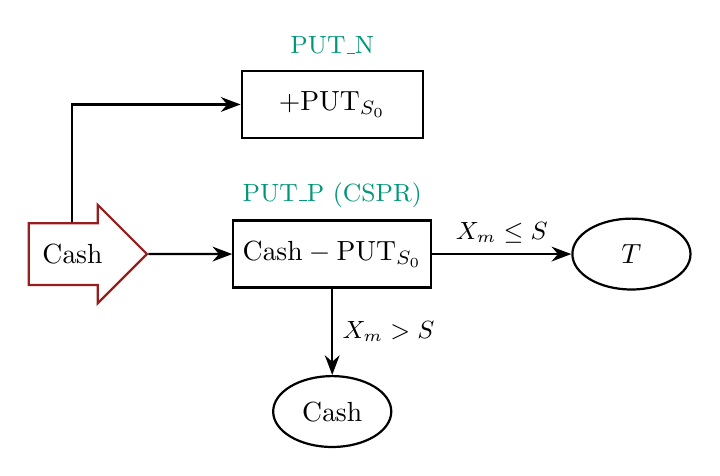
\begin{tikzpicture}[
  font=\sffamily,
  box/.style={draw, rectangle, minimum width=2.3cm, minimum height=0.85cm, align=center, line width=0.8pt},
  ell/.style={draw, ellipse, minimum width=1.5cm, minimum height=0.9cm, align=center, line width=0.8pt},
  >={Stealth[length=2.5mm]},
  arrline/.style={->, line width=0.8pt},
]
\node[single arrow, draw, line width=0.8pt, minimum width=1.25cm, minimum height=1.5cm,
      single arrow head extend=1.5mm, color=wbred] (Centry) at (0,1.3) {\color{black}$\mathrm{Cash}$};
\node[box] (putS0) at (3.3,3.2) {$+\mathrm{PUT}_{S_0}$};
\node[font=\small, color=wbgreen] at (3.3,3.95) {$\PN$};
\node[box] (cspr) at (3.3,1.3) {$\mathrm{Cash}-\mathrm{PUT}_{S_0}$};
\node[font=\small, color=wbgreen] at (3.3,2.05) {$\PP$ (CSPR)};
\node[ell] (Tres) at (7.1,1.3) {$T$};
\node[ell] (cashRes) at (3.3,-0.7) {$\mathrm{Cash}$};
\draw[arrline] (Centry.north) |- (putS0.west);
\draw[arrline] (Centry.east) -- (cspr.west);
\draw[arrline] (cspr.east) -- node[pos=0.5,above,font=\small] {$X_m\le S$} (Tres.west);
\draw[arrline] (cspr.south) -- node[pos=0.5,right,font=\small] {$X_m>S$} (cashRes.north);
\end{tikzpicture}
\end{center}

We start with \emph{cash} collateral: $C=S_0$. At the base strike $S_0$ this cash is
tokenized into two ERC-20 tranches---a right $N$ and a residual $P$:
\[
C = (N,P) \;\longmapsto\; \PN\ \text{(long-put token)} \;+\; \PP\ \text{(cash-secured-put residual)} .
\]

\textbf{(a) Splitting.} At $S_0$ the cash splits into the cash-secured-put residual (the
cash minus the written put) and the put right:
\begin{align}
C &= (C-\Put_{S_0}) + \Put_{S_0},\\
C &= \PPat{S_0} + \PNat{S_0}.
\end{align}
$\PPat{S_0}=C-\Put_{S_0}$ is the cash-secured-put leg---hold cash, short the $S_0$ put, so
it is obligated to buy the underlying below $S_0$. $\PNat{S_0}=\Put_{S_0}$ is the long-put
leg---the bearish downside below $S_0$, collateralized by the residual holder.

\textbf{(b) Settlement.} At maturity each token clears to a closed form:
\begin{align}
\PNat{S_0}(X_m) &= \pos{S_0-X_m}=\max(0,S_0-X_m),\\
\PPat{S_0}(X_m) &= S_0-\pos{S_0-X_m}=\min(X_m,S_0).
\end{align}
The cash-secured-put leg converts the cash into the underlying $T$ when the put is assigned
($X_m\le S_0$) and keeps the cash $S_0$ otherwise. The two legs conserve to the fixed cash:
\begin{align}
\PPat{S_0}(X_m)+\PNat{S_0}(X_m)=\min(X_m,S_0)+\pos{S_0-X_m}=S_0=C.
\end{align}
In cash-collateral units ($C=S_0$),
\[
\PPat{S_0}^{\,C}=\min\!\left(1,\tfrac{X_m}{S_0}\right)C,
\qquad
\PNat{S_0}^{\,C}=\max\!\left(0,1-\tfrac{X_m}{S_0}\right)C.
\]

\textbf{(c) Settlement charts.} The two legs are the standard long-put and cash-secured-put
payoffs (USD settlement value vs.\ underlying price $X_m$):

\begin{center}
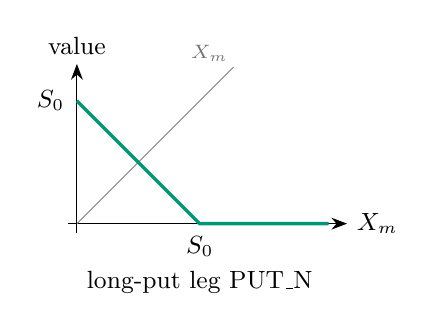
\begin{tikzpicture}[scale=0.78,>={Stealth[length=2mm]},font=\small]
  \draw[->] (-0.15,0) -- (4.4,0) node[right]{$X_m$};
  \draw[->] (0,-0.15) -- (0,2.6) node[above]{value};
  \draw[black!45] (0,0) -- (2.55,2.55) node[black!55,font=\scriptsize,above left=-2pt]{$X_m$};
  \node[below] at (2,-0.05) {$S_0$};
  \node[left] at (-0.05,2) {$S_0$};
  \draw[wbgreen,very thick] (0,2) -- (2,0) -- (4.1,0);
  \node[below] at (2.0,-0.62) {long-put leg $\PN$};
\end{tikzpicture}
\hspace{0.9cm}
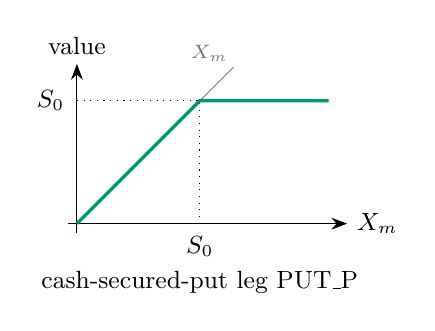
\begin{tikzpicture}[scale=0.78,>={Stealth[length=2mm]},font=\small]
  \draw[->] (-0.15,0) -- (4.4,0) node[right]{$X_m$};
  \draw[->] (0,-0.15) -- (0,2.6) node[above]{value};
  \draw[black!45] (0,0) -- (2.55,2.55) node[black!55,font=\scriptsize,above left=-2pt]{$X_m$};
  \draw[dotted] (2,0) -- (2,2);
  \draw[dotted] (0,2) -- (2,2);
  \node[below] at (2,-0.05) {$S_0$};
  \node[left] at (-0.05,2) {$S_0$};
  \draw[wbgreen,very thick] (0,0) -- (2,2) -- (4.1,2);
  \node[below] at (2.0,-0.62) {cash-secured-put leg $\PP$};
\end{tikzpicture}
\end{center}

% ---------------------------------------------------------------------
\subsection{Put-Side Recursive Split \& Bear Put Spread}
% ---------------------------------------------------------------------

\begin{center}
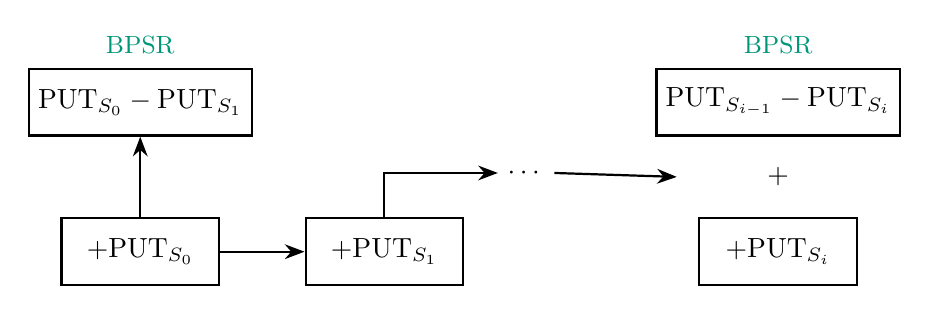
\begin{tikzpicture}[
  font=\sffamily,
  box/.style={draw, rectangle, minimum width=2.0cm, minimum height=0.85cm, align=center, line width=0.8pt},
  >={Stealth[length=2.5mm]},
  arrline/.style={->, line width=0.8pt},
]
\node[box] (putS0) at (0,0) {$+\mathrm{PUT}_{S_0}$};
\node[box] (bpsr1) at (0,1.9) {$\mathrm{PUT}_{S_0}-\mathrm{PUT}_{S_1}$};
\node[font=\small,color=wbgreen] at (0,2.62) {BPSR};
\node[box] (putS1) at (3.1,0) {$+\mathrm{PUT}_{S_1}$};
\node (pcdots) at (4.9,1.0) {$\cdots$};
\node[box] (bpsr2top) at (8.1,1.9) {$\mathrm{PUT}_{S_{i-1}}-\mathrm{PUT}_{S_i}$};
\node[font=\small,color=wbgreen] at (8.1,2.62) {BPSR};
\node[box] (bpsr2bot) at (8.1,0) {$+\mathrm{PUT}_{S_i}$};
\node at (8.1,0.95) {$+$};
\draw[arrline] (putS0.east) -- (putS1.west);
\draw[arrline] (putS0.north) -- (bpsr1.south);
\draw[arrline] (putS1.north) |- (pcdots.west);
\draw[arrline] (pcdots.east) -- ($(bpsr2top.west)!0.5!(bpsr2bot.west)$);
\end{tikzpicture}
\end{center}

The long-put token $\PN$ is itself split at the next rung. For a put ladder with
\emph{decreasing} strikes $S_0>S_1>\cdots>S_n$, each higher-strike put right splits into a
capped bear-put-spread residual plus the lower-strike put carried further down the ladder. The
put right is tokenized into a further right $N$ and a residual $P$:
\[
\PN = (N,P) \;\longmapsto\; \PNN\ \text{(lower-strike tail put)} \;+\; \PNP\ \text{(bear-put-spread residual)} .
\]

\textbf{(a) Splitting.} For $i=0,\dots,n-1$, the put right $\PNat{S_i}$ is split at the
next (lower) strike $S_{i+1}$:
\begin{align}
\PNat{S_i} &=(\Put_{S_i}-\Put_{S_{i+1}})+\Put_{S_{i+1}},\\
\PNat{S_i} &=\PNPi{S_{i+1}}+\PNNi{S_{i+1}}.
\end{align}
$\PNPi{S_{i+1}}$ is the bear-put-spread residual (long the $S_i$ put, short the $S_{i+1}$
put); $\PNNi{S_{i+1}}$ is the lower-strike tail put --- itself the put right $\PNat{S_{i+1}}$
handed to the next rung, which splits again.

\textbf{(b) Settlement.}
\begin{align}
\PNPi{S_{i+1}}(X_m) &=\pos{S_i-X_m}-\pos{S_{i+1}-X_m}
=\min\!\left(\max(0,S_i-X_m),\,S_i-S_{i+1}\right),\\
\PNNi{S_{i+1}}(X_m) &=\pos{S_{i+1}-X_m}=\max(0,S_{i+1}-X_m).
\end{align}
Since the put strikes decrease ($S_i>S_{i+1}$), $S_i-S_{i+1}>0$: the spread residual is
non-negative and capped at $S_i-S_{i+1}$.

\textbf{(c) Settlement charts.} The bear-spread leg is capped between adjacent strikes; the
tail put is an ordinary long put struck at $S_{i+1}$:

\begin{center}
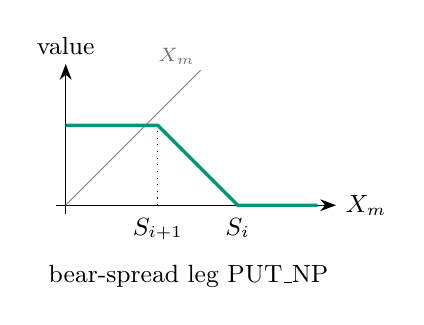
\begin{tikzpicture}[scale=0.78,>={Stealth[length=2mm]},font=\small]
  \draw[->] (-0.15,0) -- (4.4,0) node[right]{$X_m$};
  \draw[->] (0,-0.15) -- (0,2.3) node[above]{value};
  \draw[black!45] (0,0) -- (2.2,2.2) node[black!55,font=\scriptsize,above left=-2pt]{$X_m$};
  \draw[dotted] (1.5,0) -- (1.5,1.3);
  \node[below] at (1.5,-0.05) {$S_{i+1}$};
  \node[below] at (2.8,-0.05) {$S_i$};
  \draw[wbgreen,very thick] (0,1.3) -- (1.5,1.3) -- (2.8,0) -- (4.1,0);
  \node[below,align=center] at (2.0,-0.82) {bear-spread leg $\PNP$};
\end{tikzpicture}
\hspace{0.9cm}
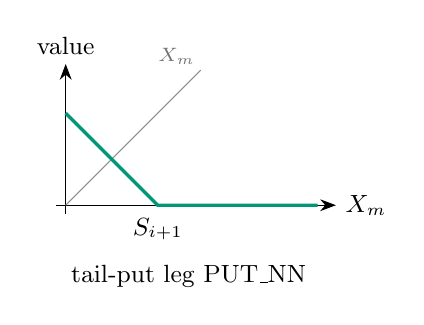
\begin{tikzpicture}[scale=0.78,>={Stealth[length=2mm]},font=\small]
  \draw[->] (-0.15,0) -- (4.4,0) node[right]{$X_m$};
  \draw[->] (0,-0.15) -- (0,2.3) node[above]{value};
  \draw[black!45] (0,0) -- (2.2,2.2) node[black!55,font=\scriptsize,above left=-2pt]{$X_m$};
  \node[below] at (1.5,-0.05) {$S_{i+1}$};
  \draw[wbgreen,very thick] (0,1.5) -- (1.5,0) -- (4.1,0);
  \node[below,align=center] at (2.0,-0.82) {tail-put leg $\PNN$};
\end{tikzpicture}
\end{center}

% ---------------------------------------------------------------------
\subsection{Put-Side Conservation: Combined Chart and Table}
% ---------------------------------------------------------------------

After recursively splitting to $S_n$, the full put-side ladder identity is
\begin{align}
S_0
&=\CSPR(X_m)+\sum_{i=1}^{n}\BPSR_{S_i}(X_m)+\Put_{S_n}(X_m),\\
&=\min(X_m,S_0)
+\sum_{i=1}^{n}\left[\pos{S_{i-1}-X_m}-\pos{S_i-X_m}\right]
+\pos{S_n-X_m},\\
&=\min(X_m,S_0)
+\sum_{i=1}^{n}\min\!\left(\max(0,S_{i-1}-X_m),S_{i-1}-S_i\right)
+\max(0,S_n-X_m).
\end{align}
The right-leg sum is telescoping:
\begin{align}
\sum_{i=1}^{n}\left[\pos{S_{i-1}-X_m}-\pos{S_i-X_m}\right]
+\pos{S_n-X_m}
=\pos{S_0-X_m},
\end{align}
so $\min(X_m,S_0)+\pos{S_0-X_m}=S_0$: the tranches always sum back to the cash collateral.

\textbf{Numerical check.} Parameters $C=S_0=2000$, $S_1=1500$, with
\begin{align}
\PP &=\min(X_m,2000),\\
\PNP &=\min\!\left(\max(0,2000-X_m),500\right),\\
\PNN &=\max(0,1500-X_m).
\end{align}

\begin{center}
\begin{tabular}{rrrrr}
\toprule
$X_m$ & $\PP$ & $\PNP$ & $\PNN$ & Total \\
\midrule
3600 & 2000 & 0 & 0 & 2000 \\
2600 & 2000 & 0 & 0 & 2000 \\
2500 & 2000 & 0 & 0 & 2000 \\
2000 & 2000 & 0 & 0 & 2000 \\
1700 & 1700 & 300 & 0 & 2000 \\
1500 & 1500 & 500 & 0 & 2000 \\
1000 & 1000 & 500 & 500 & 2000 \\
900 & 900 & 500 & 600 & 2000 \\
\bottomrule
\end{tabular}
\end{center}

\textbf{Combined chart.} Stacking the tokens at every price fills exactly up to the
\emph{flat} line $S_0$ --- the put-side total is fixed cash, the key asymmetry with the
call side ($S_0=2000$, $S_1=1500$):

\begin{center}
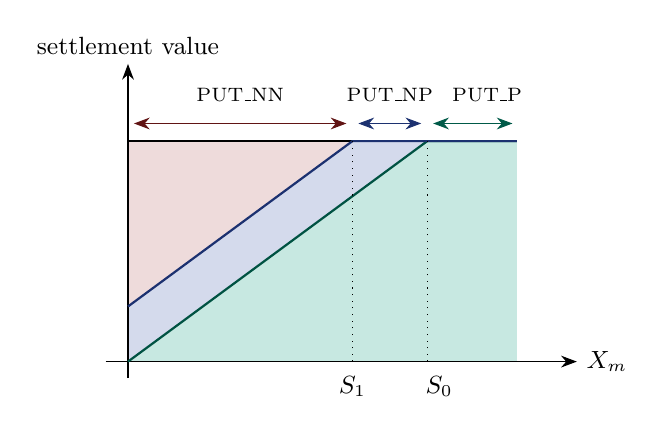
\begin{tikzpicture}[xscale=1.9,yscale=1.4,>={Stealth[length=2mm]},font=\small]
  % stacked bands (cumulative): CSPR, then +BPSR, then +tail = S_0
  \fill[wbgreen!22] (0,0) -- (2,2) -- (2.6,2) -- (2.6,0) -- cycle;
  \fill[wbblue!20]  (0,0) -- (2,2) -- (1.5,2) -- (0,0.5) -- cycle;
  \fill[wbred!16]   (0,0.5) -- (1.5,2) -- (0,2) -- cycle;
  % axes
  \draw[->] (-0.15,0) -- (3.0,0) node[right]{$X_m$};
  \draw[->] (0,-0.15) -- (0,2.7) node[above]{settlement value};
  % total (flat at S_0) --- the conserved cash
  \draw[black,thick] (0,2) -- (2.6,2);
  % cumulative boundary lines
  \draw[wbgreen!55!black,thick] (0,0) -- (2,2) -- (2.6,2);
  \draw[wbblue!70!black,thick]  (0,0.5) -- (1.5,2) -- (2.6,2);
  % strike ticks
  \draw[dotted] (1.5,0) -- (1.5,2); \node[below] at (1.5,-0.05) {$S_1$};
  \draw[dotted] (2,0) -- (2,2);     \node[below] at (2.08,-0.05) {$S_0$};
  % band labels above the chart: each <-> spans the X_m range where that token tops out at S_0
  \draw[<->,wbred!65!black]   (0.04,2.16) -- (1.46,2.16);
  \node[font=\scriptsize] at (0.75,2.42) {$\PNN$};
  \draw[<->,wbblue!70!black]  (1.54,2.16) -- (1.96,2.16);
  \node[font=\scriptsize] at (1.75,2.42) {$\PNP$};
  \draw[<->,wbgreen!60!black] (2.04,2.16) -- (2.57,2.16);
  \node[font=\scriptsize] at (2.4,2.42) {$\PP$};
\end{tikzpicture}
\end{center}

% =====================================================================
\clearpage
\section{Wheeling Strategy}
% =====================================================================

\begin{figure}[H]
\centering
\resizebox{\textwidth}{!}{%
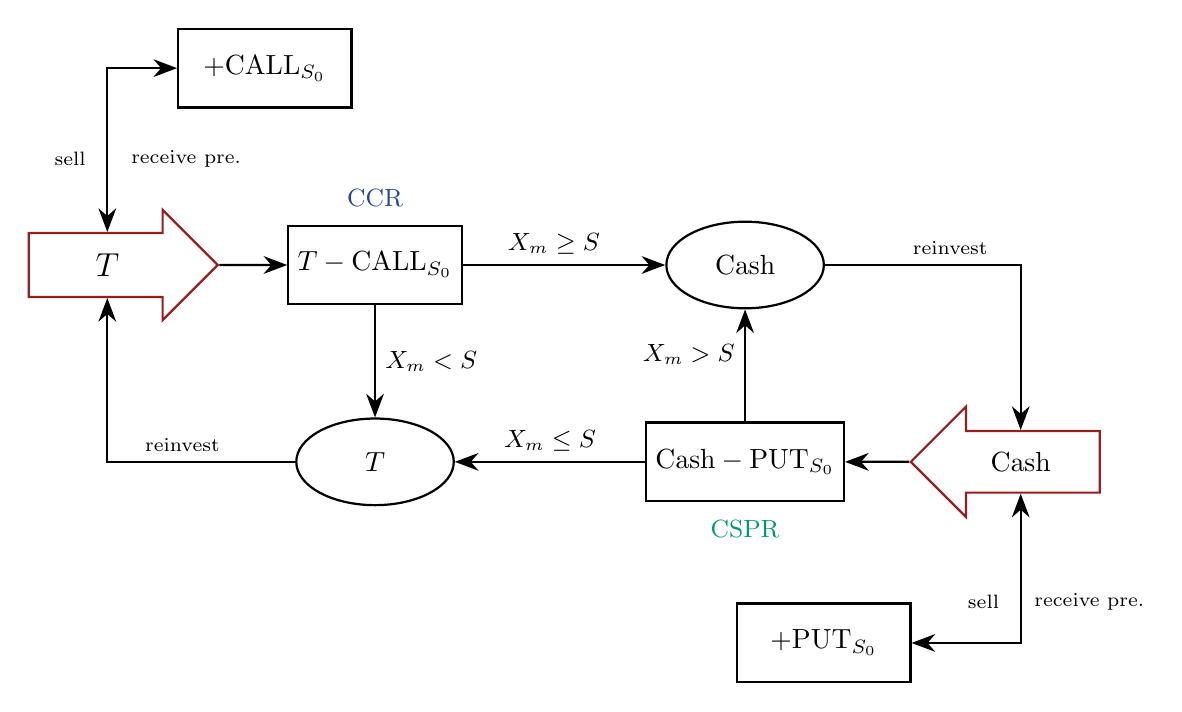
\begin{tikzpicture}[
  font=\sffamily,
  box/.style={draw, rectangle, minimum width=2.2cm, minimum height=1cm, align=center, line width=0.8pt},
  ell/.style={draw, ellipse, minimum width=2cm, minimum height=1.1cm, align=center, line width=0.8pt},
  >={Stealth[length=3mm]},
  arrline/.style={->, line width=0.8pt},
]

% ============ +CALL box (base-split call right) ============
\node[box] (callS0) at (2.6,7.4) {$+\mathrm{CALL}_{S_0}$};

% ============ Entry arrow T (big arrow, left) ============
\node[single arrow, draw, line width=0.8pt, minimum width=1.4cm, minimum height=2.4cm,
      single arrow head extend=2mm, color=wbred, rotate=0] (Tentry) at (0.6,4.9) {\color{black}\large $T$};

% ============ CCR: T - CALL_s0 ============
\node[box] (ccr) at (4.0,4.9) {$T-\mathrm{CALL}_{S_0}$};
\node[align=center, font=\small, color=wbblue] at (4.0,5.75) {CCR};

% ============ Cash ellipse ============
\node[ell] (cash1) at (8.7,4.9) {$\mathrm{Cash}$};

% ============ T ellipse (lower) ============
\node[ell] (Tell) at (4.0,2.4) {$T$};

% ============ CSPR: Cash - PUT_s0 ============
\node[box] (cspr) at (8.7,2.4) {$\mathrm{Cash}-\mathrm{PUT}_{S_0}$};
\node[align=center, font=\small, color=wbgreen] at (8.7,1.55) {CSPR};

% ============ Cash entry arrow (right) ============
\node[single arrow, draw, line width=0.8pt, minimum width=1.4cm, minimum height=2.4cm,
      single arrow head extend=2mm, color=wbred, shape border rotate=180] (cashentry) at (12.2,2.4) {\color{black}$\mathrm{Cash}$};

% ============ +PUT box (base-split put right) ============
\node[box] (putS0) at (9.7,0.1) {$+\mathrm{PUT}_{S_0}$};

% ===================== ARROWS =====================

% T <-> +CALL_s0 : single double-headed L line (up then right)
\draw[<->,line width=0.8pt] (Tentry.north) |- (callS0.west);
\node[anchor=east,font=\scriptsize] at (0.45,6.25) {sell};
\node[anchor=west,font=\scriptsize] at (0.78,6.25) {receive pre.};

% Entry T -> CCR box (the covered-call residual)
\draw[arrline] (Tentry.east) -- (ccr.west);

% CCR -> Cash  (Xm >= S)
\draw[arrline] (ccr.east) -- node[pos=0.45, above, font=\small] {$X_m\ge S$} (cash1.west);

% CCR -> T ellipse (Xm < S)  downward
\draw[arrline] (ccr.south) -- node[pos=0.5, right, font=\small] {$X_m<S$} (Tell.north);

% Cash clearing result reinvested via the cash entry
\draw[arrline] (cash1.east) -| node[pos=0.32,above,font=\scriptsize]{reinvest} (cashentry.north);

% cashentry -> CSPR
\draw[arrline] (cashentry.west) -- (cspr.east);

% CSPR -> T ellipse  (Xm <= S)
\draw[arrline] (cspr.west) -- node[pos=0.5, above, font=\small] {$X_m\le S$} (Tell.east);

% CSPR -> Cash (Xm > S) upward
\draw[arrline] (cspr.north) -- node[pos=0.6, left, font=\small] {$X_m>S$} (cash1.south);

% Cash <-> +PUT_s0 : single double-headed L line (down then left)
\draw[<->,line width=0.8pt] (cashentry.south) |- (putS0.east);
\node[anchor=east,font=\scriptsize] at (12.05,0.625) {sell};
\node[anchor=west,font=\scriptsize] at (12.25,0.625) {receive pre.};

% T clearing result reinvested via the T entry
\draw[arrline] (Tell.west) -| node[pos=0.3,above,font=\scriptsize]{reinvest} (Tentry.south);

\end{tikzpicture}%
}
\caption{The wheel: a state machine over the underlying state $T$ and the cash state.
Red arrows are entry points; each state splits into an obligation residual ($P$) and a
right ($N$). The covered-call residual ($\CCR$) and its mirror the cash-secured-put
residual ($\CSPR$) move collateral between the $T$ and Cash states at maturity according
to $X_m$ vs.\ the strike $S$; each clearing re-mints collateral into the opposite state.
The right legs $+\mathrm{CALL}_{S_0}$ and $+\mathrm{PUT}_{S_0}$ feed the call/put ladders
of Sections~3--4.}
\label{fig:ladder}
\end{figure}

The wheel cycles collateral between the underlying state $T$ and cash. Each red entry
splits a state into a residual ($\CCR$ or $\CSPR$) and a right that is sold for premium; at
maturity $\CCR$ converts $T$ to cash when $X_m\ge S$ (and keeps $T$ otherwise), while its
mirror $\CSPR$ converts cash to $T$ when $X_m\le S$ (and keeps cash otherwise). Each
clearing re-mints collateral into the opposite state, ready to be re-entered at a new
strike---the reinvest loop. The right legs $\CN$/$\PN$ feed the ladders of Sections~3--4;
closed forms follow below.

\subsection*{Equations referenced in the diagram}

\textit{Base splits (one maturity step):}
\[
T = \underbrace{(T-\Call)}_{\CP} + \underbrace{\Call}_{\CN},
\qquad
\mathrm{Cash} = \underbrace{(\mathrm{Cash}-\Put)}_{\PP} + \underbrace{\Put}_{\PN}.
\]

\textit{Entry-split weights} (token / cash units; here $S$ denotes the base strike $S_0$ and $X_m$ the terminal price):
\begin{align*}
\CP &= \min\!\left(1,\tfrac{S}{X_m}\right)T, & \CN &= \max\!\left(0,1-\tfrac{S}{X_m}\right)T,\\
\PP &= \min\!\left(1,\tfrac{X_m}{S}\right)C, & \PN &= \max\!\left(0,1-\tfrac{X_m}{S}\right)C.
\end{align*}

\textit{Per-bucket spread and tail payoffs:}
\begin{align*}
\CNPi{S_i} &= \min\!\big(\max(0,X_m-S_{i-1}),\,S_i-S_{i-1}\big), & \CNNi{S_i} &= \max(0,X_m-S_i),\\
\PNPi{S_i} &= \min\!\big(\max(0,S_{i-1}-X_m),\,S_{i-1}-S_i\big), & \PNNi{S_i} &= \max(0,S_i-X_m).
\end{align*}

% =====================================================================
\section{Summary}
% =====================================================================

\subsection*{Compact identities}

\textit{Call side, increasing strikes $S_0<S_1<\cdots<S_n$ (conserves to $X_m$):}
\begin{align}
T
&= \underbrace{\min(X_m,S_0)}_{\text{covered-call residual}}
+ \sum_{i=0}^{n}\underbrace{\min\!\left(\max(0,X_m-S_{i}),S_{i+1}-S_{i}\right)}_{\text{bull call spread residual}}
+ \underbrace{\max(0,X_m-S_n)}_{\text{tail call}}.
\end{align}

\textit{Put side, decreasing strikes $S_0>S_1>\cdots>S_n$ (conserves to $S_0$):}
\begin{align}
C
&= \underbrace{\min(X_m,S_0)}_{\text{cash-secured-put residual}}
+ \sum_{i=0}^{n}\underbrace{\min\!\left(\max(0,S_{i}-X_m),S_{i}-S_{i+1}\right)}_{\text{bear put spread residual}}
+ \underbrace{\max(0,S_n-X_m)}_{\text{tail put}}.
\end{align}

\subsection*{Tranche reference}

\begin{longtable}{l @{\hspace{2.2em}} l @{\hspace{2.2em}} l}
\toprule
Ticker & Meaning & Formula \\
\midrule
$\CP$ / $\CCR$       & Covered-call residual      & $\min(X_m,S_0)$ \\
$\CN$                & Call right (long call)     & $\max(0,X_m-S_0)$ \\
$\CNP$ / $\BCSR_{S_i}$ & Bull call spread residual  & $\min(\max(0,X_m-S_{i-1}),\,S_i-S_{i-1})$ \\
$\CNN$               & Higher-strike tail call    & $\max(0,X_m-S_i)$ \\
$\PP$ / $\CSPR$      & Cash-secured-put residual  & $\min(X_m,S_0)$ \\
$\PN$                & Put right (long put)       & $\max(0,S_0-X_m)$ \\
$\PNP$ / $\BPSR_{S_i}$ & Bear put spread residual   & $\min(\max(0,S_{i-1}-X_m),\,S_{i-1}-S_i)$ \\
$\PNN$               & Lower-strike tail put      & $\max(0,S_i-X_m)$ \\
\bottomrule
\end{longtable}

\end{document}
